\section{Third Proposed Methodology}\label{sec:6_third_proposed_approach}

This section introduces the Heterogeneous Transfer Learning (HTL) algorithm tailored for non-stationary environments. HTL adeptly assimilates knowledge from both heterogeneous and homogeneous sources, operating within the framework of data streams subject to concept drift. Leveraging an online learning inductive parameter transfer strategy, HTL achieves seamless knowledge transfer. We delineate the core components and workflow of the HTL algorithm. To address the challenges intrinsic to the third approach, the focus is on three key aspects:
\begin{itemize}
	\setlength{\itemsep}{0pt}
    \setlength{\parskip}{0pt}
	\item \textbf{Heterogeneous sources:} Traditional transfer learning methods often assume homogeneity in the data distribution across source and target domains. However, in real-world scenarios, data sources may vary significantly in terms of feature space. HTL addresses this challenge by allowing knowledge transfer from sources with different dimensionalities. This means that the algorithm can effectively learn from diverse dimentionality sources, enabling a more comprehensive knowledge transfer process.
	\item \textbf{Drifted streams:} In dynamic environments, data distributions may change over time, leading to concept drift. This phenomenon poses a significant challenge for machine learning algorithms, as models trained on historical data may become obsolete as the underlying data distribution shifts. HTL incorporates a concept drift detector that continuously monitors the incoming data stream. Upon detecting a shift in the data distribution, the algorithm adapts its classifiers accordingly to ensure continued effectiveness in handling drifting streams. This dynamic adjustment mechanism allows HTL to maintain high performance even in the presence of concept drift.
	\item \textbf{Classifier performance:} Classifier performance is crucial for the overall effectiveness of the transfer learning process. HTL employs Dynamic Ensemble Selection (DES) to enhance classifier performance. DES creates a diverse ensemble of classifiers, each trained on different subsets of the data. When presented with a new data point, DES dynamically selects the most suitable classifiers from the ensemble based on its performance on similar chunk. This adaptive selection process ensures that the most appropriate classifier is chosen for each data point, leading to improved classification performance and robustness. By leveraging DES, HTL maximizes the utility of available classifiers, resulting in superior performance in non-stationary environments with heterogeneous data sources.
\end{itemize}

\subsection{HTL Description}

The aim of this section is to harness knowledge from diverse dimensional multisource domain streams. Following a similar framework to CDTL \cite{yang2021concept}, this approach employs a class-wise and domain-weighted strategy. However, HTL enhances the weight function of CDTL in a class-wise manner, as depicted in Fig. \ref{fig:6_alg1}, encompassing three phases:

\begin{itemize}
	\setlength{\itemsep}{0pt}
    \setlength{\parskip}{0pt}
	\item \textbf{Dynamic ensemble selection phase (DES Phase):}: The primary objective DES phase is to identify the optimal classifier for incoming data. This is crucial for ensuring that the selected classifier effectively aligns with the unique characteristics of the current data segment.
	\item \textbf{Drift detector phase:} After the DES phase, the method progresses to the drift detector phase, where it operates in real-time to continually monitor the data stream. This phase employs ADWIN and DDM techniques, which play a pivotal role in swiftly identifying any signs of concept drift. These techniques are designed to detect changes in the underlying data distribution over time, thus enabling the algorithm to adapt to evolving data patterns.
	\begin{figure}[H]
		\centering
		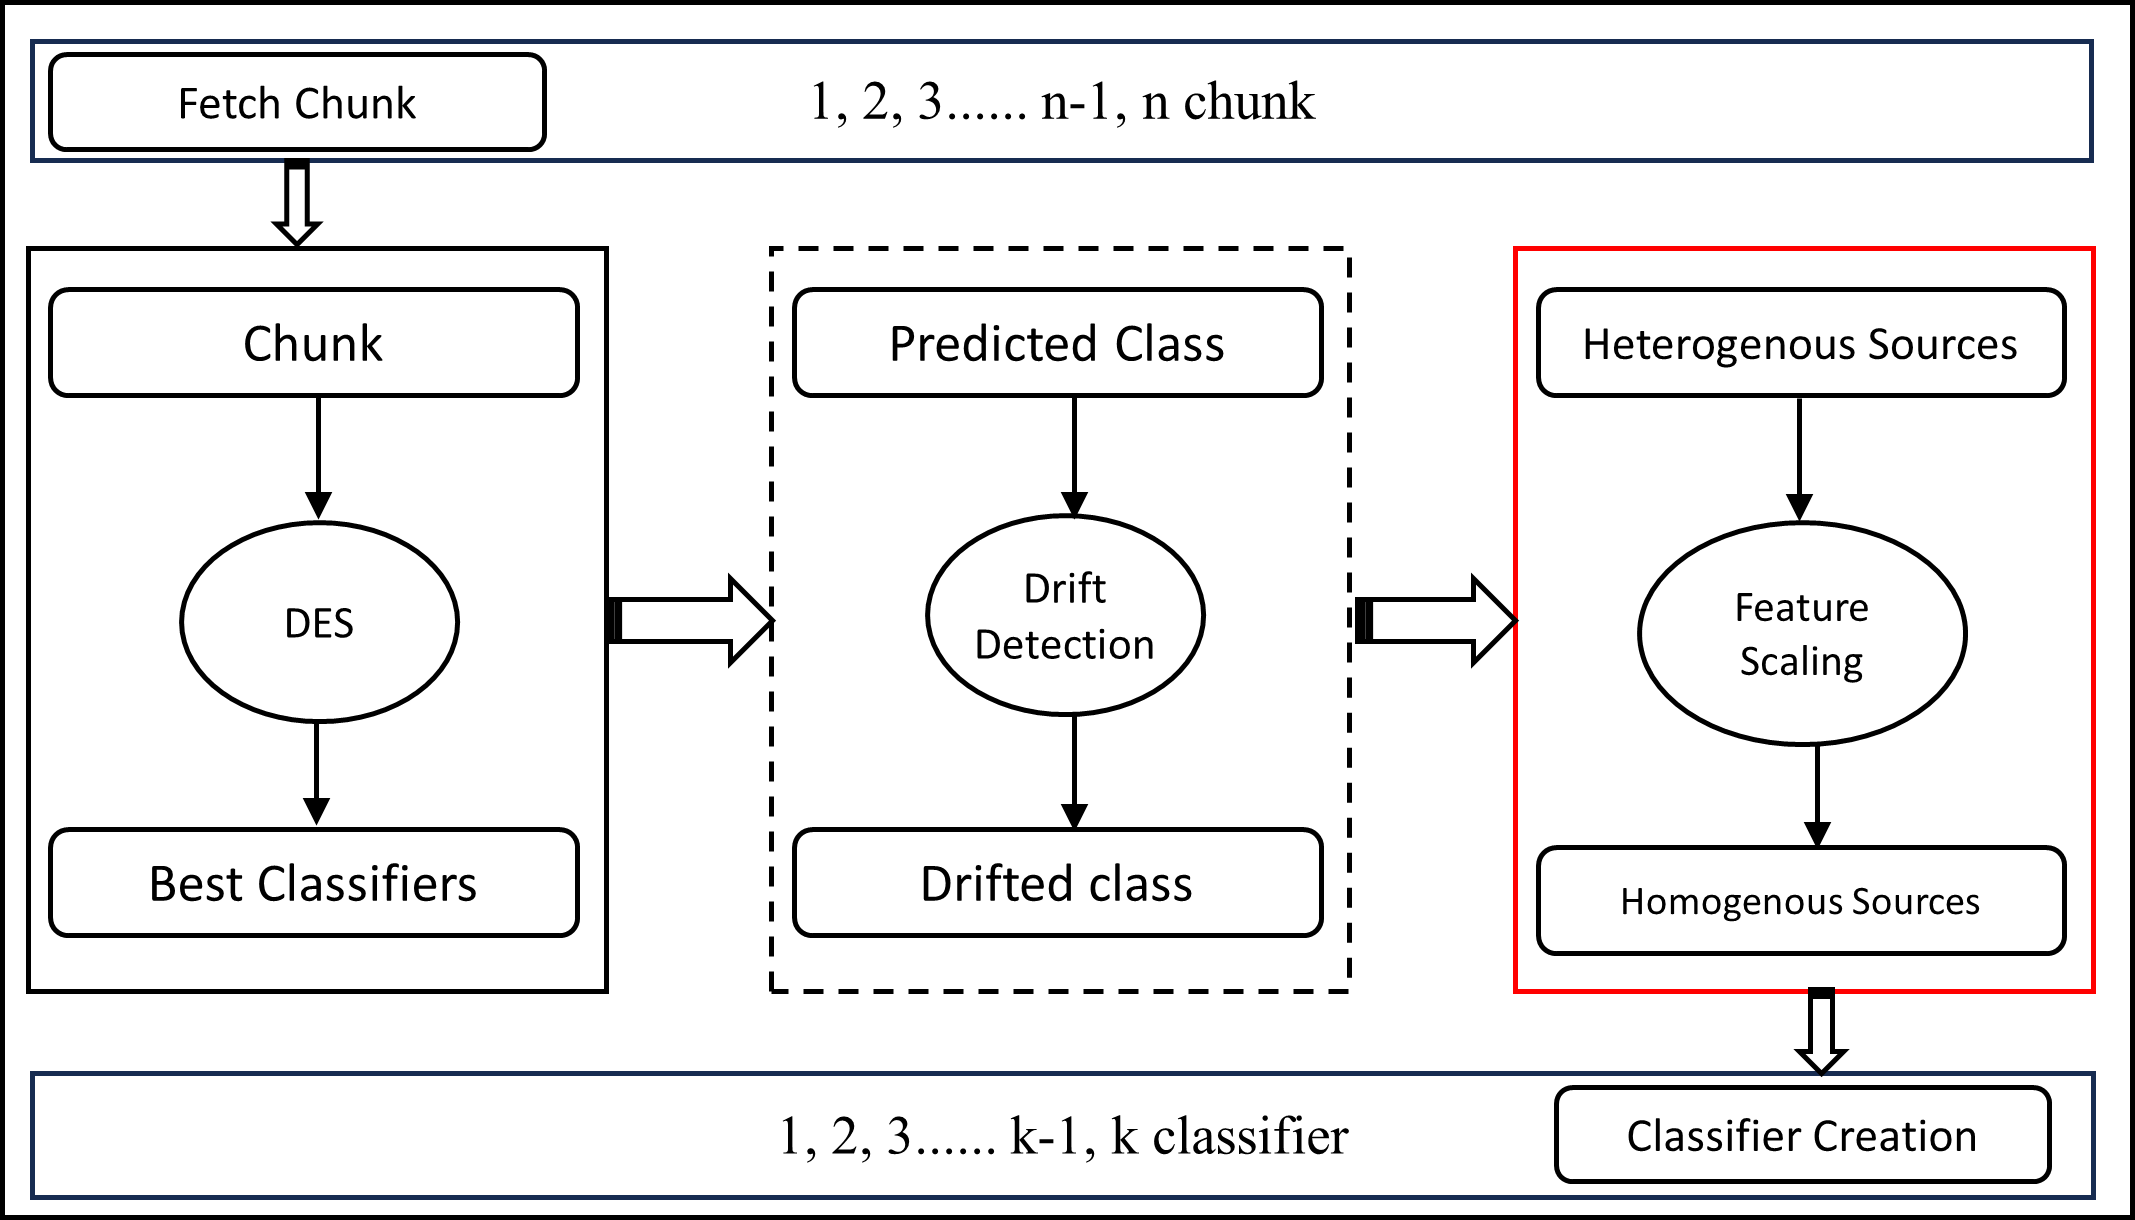
\includegraphics[width=0.8\linewidth]{6_transfer_learning/figures/alg1.png}
	  \caption{HTL Flow Diagram.}
		\label{fig:6_alg1}
	\end{figure}

	\item \textbf{Feature scaling} The concluding phase of HTL is featuring scaling, operating in real-time to harmonize the diverse dimensionalities of the multisource streams with the target dimensionality. Leveraging the eigen vector technique, this phase facilitates the transformation of data into a unified dimensionality, essential for creating new classifiers tailored to the target and domain streams. By ensuring compatibility with the learning framework, this process enhances the algorithm's effectiveness in handling diverse dimensionality streams.
\end{itemize}

\subsection{Classifier Creation Phase Description} 
Figure \ref{fig:6_alg_2} provides a comprehensive overview of the classifier creation phase, a crucial component responsible for generating new classifiers based on the current chunk of the target domain, previous classifiers, and source domain classifiers. This phase offers several advantages and perform three tasks.
\begin{itemize}
	\setlength{\itemsep}{0pt}
    \setlength{\parskip}{0pt}
	\item \textbf{Source projection:} This step involves projecting the source domain classifiers onto the current chunk of the target domain. The projection likely employs the source weight function, as described in CDTL \cite{yang2021concept}, to assign a weight to each classifier based on its relevance to the current chunk of data. This weighting mechanism ensures that classifiers from the source domains contribute appropriately to the creation of the new classifier for the target domain.
	\begin{figure}[H]
		\centering
		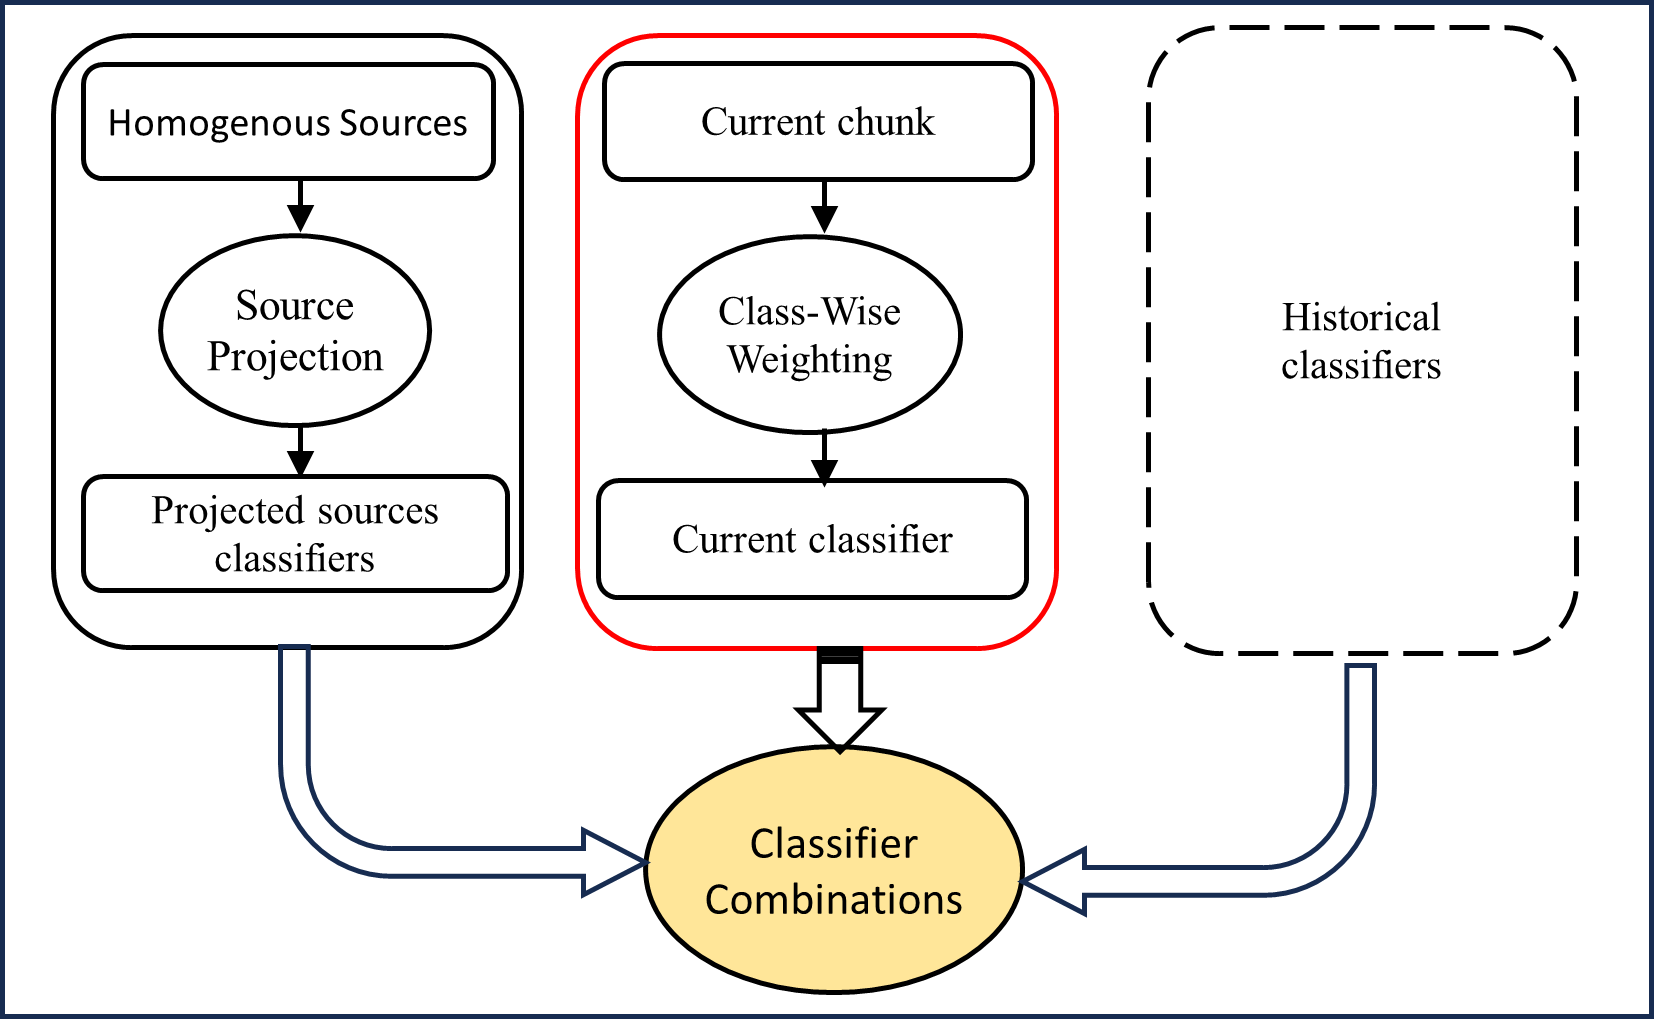
\includegraphics[width=0.8\linewidth]{6_transfer_learning/figures/alg2.png}
	  \caption{Classifier Creation Phase Flow Diagram.}
		\label{fig:6_alg_2}
	\end{figure}
	\item \textbf{Class-wise weights:} This block computes class-specific weights for each classifier using Equations \ref{eq:6_eq_1} and \ref{eq:6_eq_2} . The process involves analyzing the current chunk of the target stream (denoted as \emph{D}) and considering both correct and incorrect predictions made by each classifier where $prediction_i$ refers to the predicted class of the current instance and $c$ to the income class. These weights are crucial for determining the significance of individual classifiers across different classes. The equations facilitate the calculation of weights that reflect the classifiers' performance on specific classes, enabling the creation of a well-balanced ensemble classifier.
	\item \textbf{Classifier combination:} In this phase, the class-wise weights, along with the current chunk of data and the projected source domain classifiers, are combined to derive the final classifier. The combination process follows the details outlined in Eq. \ref{eq:6_eq_3} , where historical classifiers (denoted as \emph{H}), projected data classifiers (denoted as \emph{P}), and the classifier of the current chunk (denoted as \emph{K}) are integrated. This integration ensures that the resulting classifier incorporates contributions from both historical and projected data sources, leveraging the strengths of each to enhance predictive performance. The resulting classifier is then utilized to make predictions based on the data chunk, effectively leveraging the insights gleaned from both historical and current data sources.
\end{itemize}


\section{Mathematical Foundations of the HTL}

The proposed Heterogeneous Transfer Learning (HTL) framework incorporates several mathematical components to enhance classification performance in dynamic data streams. Below, an analysis of the key equations is provided, used to define the methodology.

The first step in the framework is calculating the \textbf{class weight} for each class \(c\) predicted by a base classifier \(k\) over a dataset \(\mathcal{D}\):

\begin{equation}
\label{eq:6_eq_1}
{classWeight}_{k,c,\mathcal{D}} = \sum_{i \in \mathcal{D}} \frac{|{prediction}_i = c|}{|\mathcal{D}|} \times \frac{|{prediction}_i \neq c|}{|\mathcal{D}|}.
\end{equation}

This formula measures the relative contribution of a classifier \(k\) to the classification of class \(c\), balancing correct and incorrect predictions within the dataset \(\mathcal{D}\).

Next, the \textbf{classifier weight} is determined by aggregating the class weights across all classes \(C\) and classifiers \(K\) for the dataset:

\begin{equation}
\label{eq:6_eq_2}
{classifierWeight} = \sum_{k \in K} \sum_{c \in C} {classWeight}_{k,c,\mathcal{D}}, \quad \text{where } \mathcal{D} = 1, 2, 3, \dots, N.
\end{equation}

This aggregation quantifies the overall performance of a classifier \(k\) in the context of all classes in the dataset.

Finally, the \textbf{prediction ensemble} combines predictions from primary sources \(P\), heterogeneous sources \(H\), and the current classifier \(k\) for a given data chunk:

\begin{equation}
\label{eq:6_eq_3}
{Prediction}_{p,H,k,chunk} = \sum_{p \in P} {{prediction}^{p}_{chunk}} + \sum_{h \in H} {{prediction}^{h}_{chunk}} + {prediction}^{k}_{chunk}.
\end{equation}

This equation ensures that the final prediction leverages diverse knowledge sources, including heterogeneous and primary streams, to achieve robust and accurate predictions for the data chunk.

These mathematical formulations underline the HTL framework's capability to dynamically adjust to evolving data distributions and heterogeneities in multi-source streaming environments.

\subsection{HTL Algorithm Description}

As illustrated in Algorithm \ref{alg:6_alg_1}, the HTL algorithm involves several stages, beginning with training a classifier for the target stream and proceeding through various steps related to heterogeneous multisource preprocessing, classifier weighting, concept drift detection, and classifier management to ensure the performance and adaptability of the final classifier. In this section, detailed explanations of each individual step within the HTL algorithm are provided.
\begin{itemize}
	\setlength{\itemsep}{0pt}
    \setlength{\parskip}{0pt}
	\item \textbf{Converting heterogeneous multisource to homogeneous multisource:} In the initial step, the algorithm unifies the various data sources that might have different characteristics (heterogeneous multisource). This is achieved using eigenvectors and the feature count of the current chunk (line 7).
	\item \textbf{Training a new classifier for the first target chunk:} In line 8, the new classifier is trained specifically for the first chunk of the target stream. This classifier was used to predict the initial chunk of the target stream.
	\item \textbf{Calculate heterogeneous multisource weights:} The algorithm computes the weights for each heterogeneous data source. These weights are determined based on the characteristics of the data from each source and the target classifier. This weighting process helps prioritize more relevant data sources (line 9).
	\item \textbf{Calculating class-wise weights:} In line 27, the algorithm calculates class-wise weights using Equations 1 and 2. These weights were essential for determining the contribution of each class to the final classifier.
	\item \textbf{Converting homogeneous multisource to projected data source:} Line 11 involves using the weights calculated in the third step to transform the homogeneous multisource representation to a projected data source. This transformation likely uses the source weight function of CDTL \cite{yang2021concept}.
	\item \textbf{Prediction of the current chunk:} In line 16, the algorithm determines the output class using Equation 3.
	\item \textbf{Monitoring for concept drift:} The algorithm continuously monitors the performance of its predictions to detect any concept drift, a situation in which the underlying data distribution changes, potentially leading to a degradation in model performance. Line 19 has been used for this purpose.
	\item \textbf{Updating the projected multisource classifiers:}Lines 29–32 are dedicated to updating the classifiers associated with the projected multisource. It is necessary to adapt to changes in the data or to maintain the performance and relevance of the classifiers over time.
	\item \textbf{Managing the pool of classifiers:} If the pool of classifiers exceeds a predefined maximum size threshold, lines 23 and 24 indicate that a new classifier is trained, and the worst-performing classifier is removed. This process helps to maintain a manageable and effective set of classifiers.
\end{itemize}
The heterogeneous Transfer Learning (HTL) algorithm represents a significant advancement in addressing the complexities of non-stationary environments prone to concept drift. By integrating heterogeneous and homogeneous sources within dynamic data streams, HTL demonstrates remarkable adaptability and effectiveness. Through its meticulously designed workflow, HTL can efficiently handle the challenges posed by evolving data landscapes. From the initial reception of environmental data to the nuanced processing of new data chunks and vigilant monitoring of concept drift, HTL embodies a comprehensive approach to knowledge transfer and adaptation. Owing to its ability to compute class-specific weights and leverage vital classifiers, HTL offers a robust solution for navigating non-stationary environments with confidence and precision.
\begin{algorithm}[!ht]
	\DontPrintSemicolon
	\KwIn{Target domain stream \emph{stream}, heterogeneous multisource domain $\Psi$, pool of classifiers, threshold $\ell$}
		\KwData{Current chunk \emph{a}, classifiers \emph{k}, source classifiers $\psi$, projected source domain \emph{S}, target domain weights $\omega$, source domain weights $\lambda$}
		\KwOut{Prediction}
		  \For{$ \emph{stream}\ have\ chunk$ }{
				  \eIf{$\emph{a}\ is\ the\ First\ chunk$}{
				    $\Psi \gets convertSourcesToTargetDim(\Psi,\ \emph{a})$\;
				    $\emph{k} \gets  trainingNewClassifier(\emph{a})$\;
				    $\lambda \gets SourcesDomainWeights(\Psi,\ \emph{k})$\;
						 $\omega \gets classWiseWeights(\emph{K},\ \emph{a})$\;
				    $\emph{S} \gets projectedSourceDomain(\Psi,\ \lambda)$\;
				   \For{$\emph{source}\ in\ \emph{S}$}{
						 $\emph{newClassifier} \gets  trainingNewClassifier(\emph{source})$\;
				    $\psi \gets  \psi \cup\  \emph{newClassifier}$\;
			  
				   }
				   $\emph{prediction} \gets getPrediction(\emph{a},\ \emph{k},\ \psi,\ \lambda,\ \omega)$ \;
				   }{
				   $\emph{prediction} \gets getPrediction(\emph{a},\ \emph{k},\ \psi)$ \;
					   $driftResult \gets conceptDriftDetector(\emph{prediction})$ \;
			  
					  \If{ $driftResult\ have\ drift $}{
					    $\emph{newClassifier} \gets trainingNewClassifier(\emph{a})$\;
				    $\emph{k} \gets \emph{k}\ \cup \emph{newClassifier}$\;
						\If{$size(\emph{K}) \geq \ell$}{
						 $removeWorstClasssifier(\emph{k})$\;
						}
				    $\lambda \gets SourcesDomainWeights(\Psi,\ \emph{k})$\;
				    $\omega \gets classWiseWeights(\emph{K},\ \emph{a})$\;
			  
				    $\emph{S} \gets projectedSourceDomain(\Psi,\ \lambda)$\;
				   \For{$\emph{source}\ in\ \emph{S}$}{
						 $\emph{newClassifier} \gets  trainingNewClassifier(\emph{source})$\;
				    $\psi \gets  \psi \cup\  \emph{newClassifier}$\;
			  
				   }
				  
				   $\emph{prediction} \gets getPrediction(\emph{a},\ \emph{k},\ \psi,\ \lambda,\ \omega)$ \;
					 }
				  }
				  }
	\Return{$\emph{prediction}$}\;
	\caption{Flow Diagram of the Heterogeneous Transfer Learning.}
	\label{alg:6_alg_1}

\end{algorithm}
